\documentclass[]{article}
\usepackage[a4paper, total={6in, 8in}]{geometry}
\usepackage[]{amsmath}
\usepackage[]{mathrsfs}
\usepackage[]{graphicx}
\usepackage[]{setspace}
\usepackage[]{amssymb}
\usepackage[]{multicol}
\geometry{margin=1cm}
\graphicspath{ {./images/} }
\date{}
\pagenumbering{gobble}
\begin{document}
\begin{multicols}{2}
    \section*{Continuous Elementary Signal}
    \begin{spacing}{1.5}
        $rect(\dfrac{t}{\tau}) = \begin{cases}
                1\, & |t| < \dfrac{\tau}{2} \\
                0\, & |t| > \dfrac{\tau}{2}
            \end{cases}$\\
    \end{spacing}
    $u(t) = \begin{cases}
            1\, & |t| > 0 \\
            0\, & |t| < 0
        \end{cases}$ ~ $r(t) = \begin{cases}
            t\, & |t| > 0 \\
            0\, & |t| < 0
        \end{cases}$
    \section*{Unit Impulse Function}
    \begin{enumerate}
        \item $\delta(0) \rightarrow \infty$
        \item $\delta(t) = 0, t \neq \infty$
        \item $\int\limits_{-\infty}^{\infty} \delta(t)\, dt = 1$
        \item $\delta(t)$ is an even function, i.e., $\delta(t) = \delta(-t)$
    \end{enumerate}
    \begin{itemize}
        \item \textbf{Sifting} $\int\limits_{t_1}{t_2}x(t)\delta(t-t_0)\, dt = \begin{cases}
                      x(t_0)\, & t_1 < t_0 < t_2  \\
                      0\,      & \text{otherwise}
                  \end{cases}$
        \item \textbf{Sampling} $x(t)\delta(t-t_0) = x(t_0)\delta(t-t0)$
        \item \textbf{Scaling} $\delta(at+b) = \dfrac{1}{|a|} \delta(t + \dfrac{b}{a})$
    \end{itemize}
    $\dfrac{d u(t)}{dt} = \delta(t)$ ~ $\int\limits_{-\infty}^{\infty} \delta(\tau)\, d\tau = u(t)$
    \section*{Periodic Signal}
    \subsection*{Continous}
    $x(t) = x(t+nT)$ $T$ is period, $T = \dfrac{2\pi}{|\omega_0|}$\\~\\
    $z(t) = ax(t) + by(t)$  ~ $ x(t) = x(t+ kT_1)$ ~ $y(t) = y(t + lT_2)$\\~\\
    Will be Periodic if $T = kT_1 = lT_2$ where $k, l$ are integers
    \subsection*{Discrete}
    $x[n] = x[n + N] \text{ for all } n,\text{ some integer } N > 0$

    \section*{Continuous Time System}
    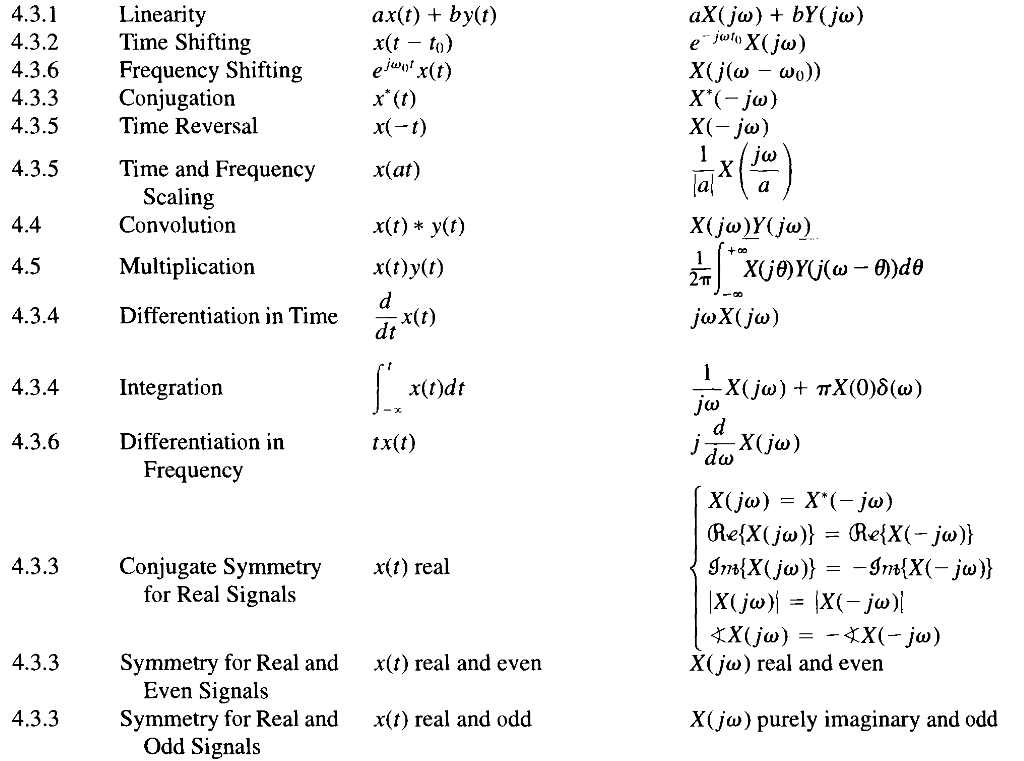
\includegraphics[scale=0.3]{continuous1.png}\\
    \section*{Discrete Elementary Signal}
    $\delta[n] = \begin{cases}
            1\, & n = 0    \\
            0\, & n \neq 0
        \end{cases}$ ~
    $u[n] = \begin{cases}
            1\, & n \geq 0 \\
            0\, & n < 0
        \end{cases} = \sum\limits_{k = 0}^{\infty} \delta[k]
    $\\\\
    $u[n] - u[n - 1] = \delta[n]$ ~ $x[n]\delta[n-k] = x[k]\delta[n-k]$\\
    $x[n] = \sum\limits_{k=-\infty}^{\infty} x[k]\delta[n-k]$
    \section*{Convolution}
    \subsection*{Continuous}
    $y(t) = \int\limits_{-\infty}^{\infty} x(\tau)h(t-\tau)\, d\tau = x(t) * h(t)$, ~ $x(t) * \delta(t-a) = x(t-a)$\\
    $x(t)*u(t) = \int\limits_{-\infty}^{\infty} x(\tau) u(t-\tau)\, d\tau = \int\limits_{-\infty}^{t} x(\tau)\, d\tau$
    \subsection*{Discrete}
    $y[n] = \sum\limits_{k = -\infty}^{\infty} x[k]h[n-k] = x[n] * h[n]$\\
    $x[n]*u[n] = \sum\limits_{k=-\infty}^{\infty} x[k]u[n-k] = \sum\limits_{k=-\infty}^{n} x[k]$

    \section*{Continuous Fourier Transform}
    $rect(\dfrac{t}{\tau}) \leftrightarrow \tau sinc(\dfrac{\omega \tau}{2})$ ~
    $e^{-\alpha t} \leftrightarrow \dfrac{1}{\alpha + j \omega}$\\
    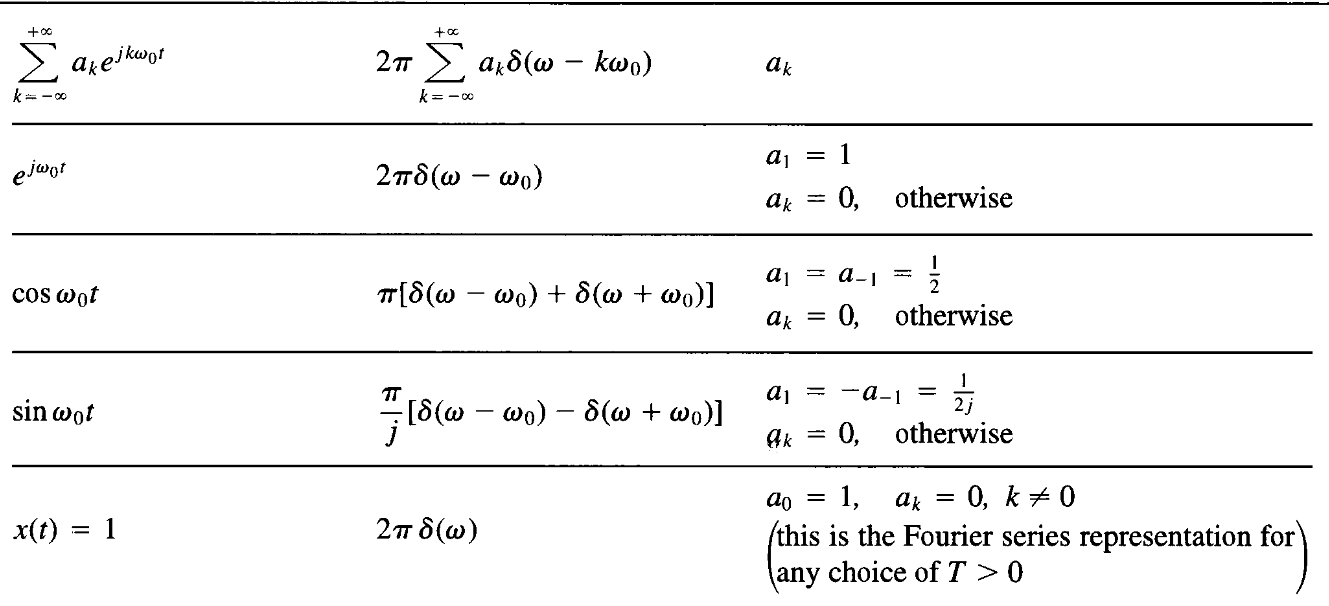
\includegraphics[scale=0.25]{continuous2.png}\\
    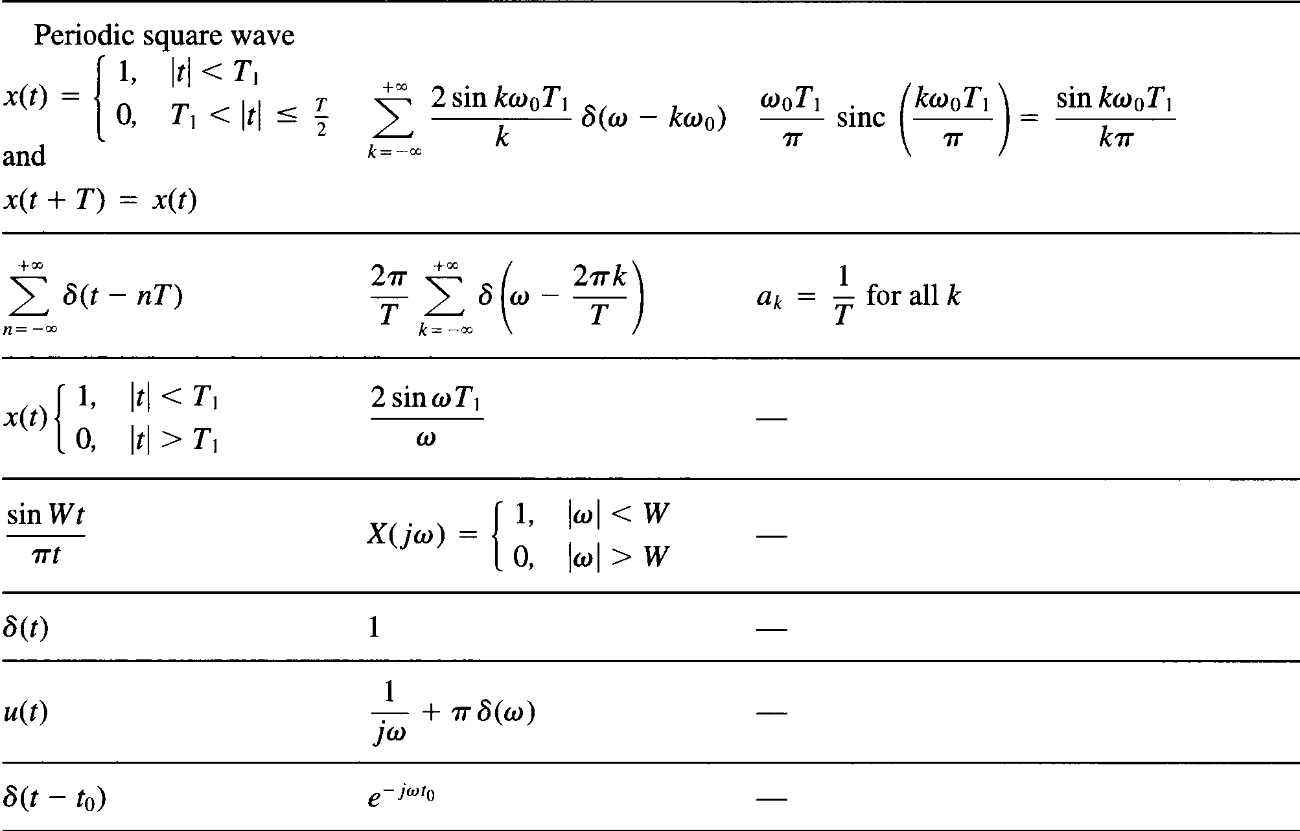
\includegraphics[scale=0.25]{continuous3.png}\\
    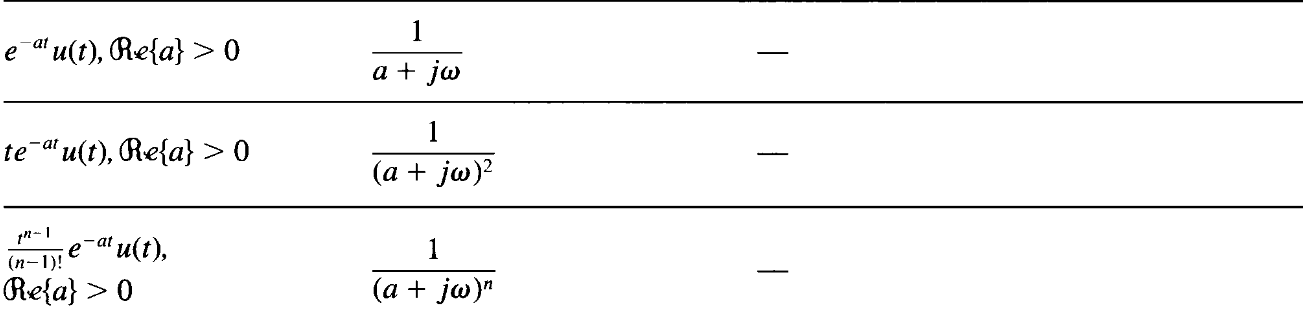
\includegraphics[scale=0.25]{continuous4.png}\\
    \newpage
    \section*{Fourier Transform for DT (DTFT)}
    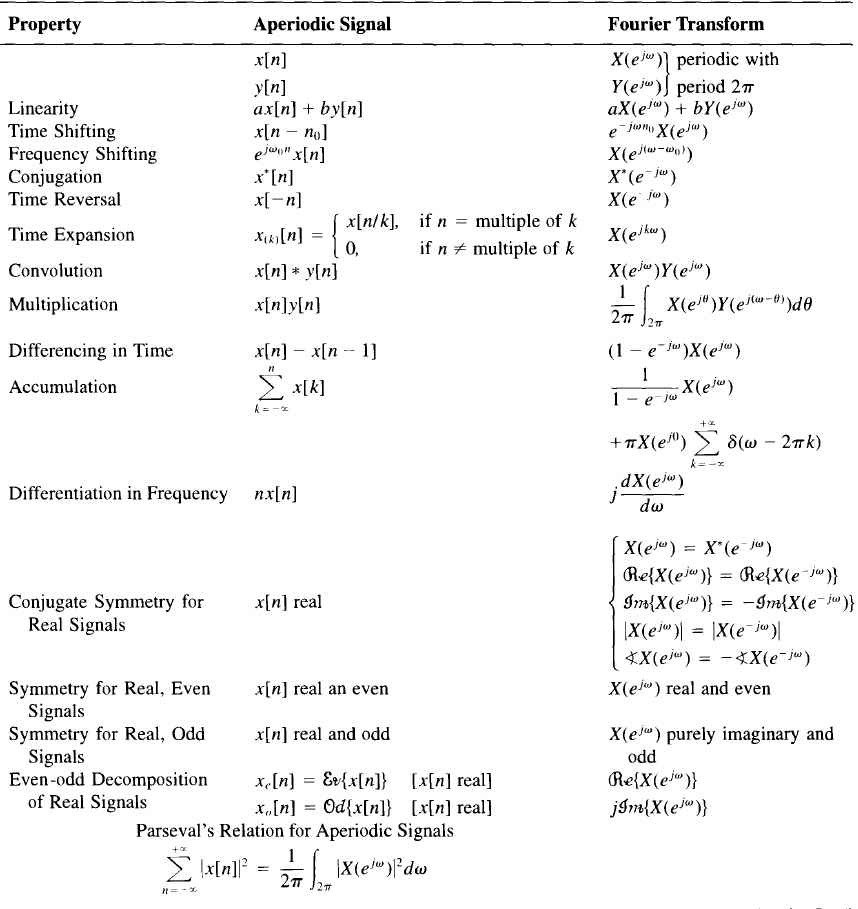
\includegraphics[scale=0.4]{discrete1.png}
    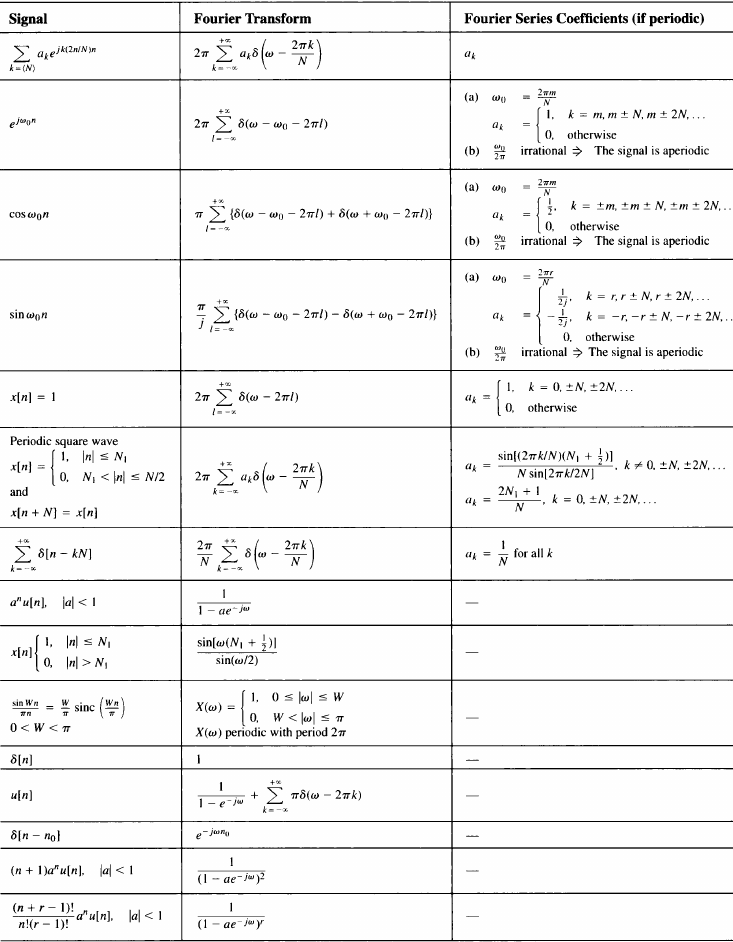
\includegraphics[scale=0.5]{discrete2.png}

    \section*{Discrete Fourier Transform (DFT)}
    \subsection*{Matrix Representation}
    $X[k] = \sum\limits_{n = 0}^{N-1} x[n]W_{n}^{nk}\,; k = 0,1,...,N-1$\\
    \subsection*{Convolution Example}
    \begin{spacing}{2.5}
        $x[n] = \{1, 2, 0 ,-1\}$ $h[n] = \{1,3,-1,2\}$ $N = 4$ $e^{\frac{-2\pi}{4}j} = -j$\\
        $X = Wx = \left[\begin{smallmatrix}
                    1 & 1  & 1  & 1  \\
                    1 & -j & -1 & j  \\
                    1 & -1 & 1  & -1 \\
                    1 & j  & -1 & -j
                \end{smallmatrix}\right]\left[\begin{smallmatrix}
                    1 \\
                    2 \\
                    0 \\
                    1
                \end{smallmatrix}\right] = \left[\begin{smallmatrix}
                    2    \\
                    1-3j \\
                    0    \\
                    1+3j
                \end{smallmatrix}\right]$\\
        $H = Wh = \left[\begin{smallmatrix}
                    1 & 1  & 1  & 1  \\
                    1 & -j & -1 & j  \\
                    1 & -1 & 1  & -1 \\
                    1 & j  & -1 & -j
                \end{smallmatrix}\right]\left[\begin{smallmatrix}
                    1  \\
                    3  \\
                    -1 \\
                    2
                \end{smallmatrix}\right] = \left[\begin{smallmatrix}
                    1    \\
                    2-5j \\
                    -1   \\
                    2+5j
                \end{smallmatrix}\right]$\\
        $Y = XH = \left[\begin{smallmatrix}
                    2       \\
                    -13-11j \\
                    0       \\
                    -13+11j
                \end{smallmatrix}\right]$ $W^{-1} = \dfrac{1}{N} W^{*}$\\
        $y = \dfrac{1}{4} \left[\begin{smallmatrix}
                    1 & 1  & 1  & 1  \\
                    1 & j  & -1 & -j \\
                    1 & -1 & 1  & -1 \\
                    1 & -j & 1  & j
                \end{smallmatrix}\right] = \left[\begin{smallmatrix}
                    2       \\
                    -13-17j \\
                    0       \\
                    -13+11j
                \end{smallmatrix}\right] = \left[\begin{smallmatrix}
                    -6 \\
                    6  \\
                    7  \\
                    -5
                \end{smallmatrix}\right]$
    \end{spacing}
    \section*{Sampling}
    \textbf{Nyquist rate} $2\omega_0$\\
    \subsection*{Impulse Train Sampling}
    $x(t)$ low pass signal and no freq. $> \omega_B$\\
    $p(t)$ periodic impulse train\\
    $T_s$ sampling period\\
    Output of the sampler $x_s(t)$\\
    Fundamental freq. (sampling freq.) of $p(t)$ is $\omega_s = \dfrac{2\pi}{T_s}$\\
    $x_s(t) = x(t)p(t) \text{ where } p(t) = \sum\limits_{n = -\infty}^{\infty} \delta(t - nT_s)$

    \subsection*{Aliasing}
    $\omega_s < 2\omega_B \rightarrow \text{Aliasing}$ \\
    Reconstructed frequency $f_p$ of signal frequency $f$ which is sampled at $f_s$\\
    $f_p = |f - kf_s|\, ;k \text{ is the rounded value of } \dfrac{f}{f_s}$

\end{multicols}
\end{document}